% Created 2024-02-09 vie 15:08
% Intended LaTeX compiler: pdflatex
\documentclass[aspectratio=169, usenames,svgnames,dvipsnames]{beamer}
\usepackage[utf8]{inputenc}
\usepackage[T1]{fontenc}
\usepackage{graphicx}
\usepackage{grffile}
\usepackage{longtable}
\usepackage{wrapfig}
\usepackage{rotating}
\usepackage[normalem]{ulem}
\usepackage{amsmath}
\usepackage{textcomp}
\usepackage{amssymb}
\usepackage{capt-of}
\usepackage{hyperref}
\usepackage{color}
\usepackage{listings}
\usepackage{mathpazo}
\usepackage{gensymb}
\usepackage{amsmath}
\usepackage{diffcoeff}
\usepackage{steinmetz}
\usepackage{mathtools}
\usepackage{fancyvrb}
\DefineVerbatimEnvironment{verbatim}{Verbatim}{fontsize=\tiny, formatcom = {\color{black!70}}}
\bibliographystyle{plain}
\usepackage{siunitx}
\sisetup{per-mode=symbol}
\sisetup{output-decimal-marker={,}}
\DeclareSIUnit{\watthour}{Wh}
\DeclareSIUnit{\wattpeak}{Wp}
\DeclareSIUnit{\watthour}{Wh}
\DeclareSIUnit{\amperehour}{Ah}
\usepackage{steinmetz}
\hypersetup{colorlinks=true, linkcolor=Blue, urlcolor=Blue}
\usepackage[symbol, perpage]{footmisc}
\parskip=5pt
\usetheme{Boadilla}
\usecolortheme{rose}
\usefonttheme{serif}
\author{\href{https://oscarperpinan.github.io}{Oscar Perpiñán Lamigueiro}}
\date{}
\title{Geometría y Radiación de los Sistemas Fotovoltaicos}
\subtitle{Energía Solar Fotovoltaica}
\institute[UPM]{Universidad Politécnica de Madrid}
\setbeamercolor{alerted text}{fg=blue!50!black} \setbeamerfont{alerted text}{series=\bfseries}
\AtBeginSubsection[]{\begin{frame}[plain]\tableofcontents[currentsubsection,sectionstyle=show/hide,subsectionstyle=show/shaded/hide]\end{frame}}
\AtBeginSection[]{\begin{frame}[plain]\tableofcontents[currentsection,hideallsubsections]\end{frame}}
\beamertemplatenavigationsymbolsempty
\setbeamertemplate{footline}[frame number]
\setbeamertemplate{itemize items}[triangle]
\setbeamertemplate{enumerate items}[circle]
\setbeamertemplate{section in toc}[circle]
\setbeamertemplate{subsection in toc}[circle]
\hypersetup{
 pdfauthor={\href{https://oscarperpinan.github.io}{Oscar Perpiñán Lamigueiro}},
 pdftitle={Geometría y Radiación de los Sistemas Fotovoltaicos},
 pdfkeywords={},
 pdfsubject={},
 pdfcreator={Emacs 29.1 (Org mode 9.4.6)}, 
 pdflang={Spanish}}
\begin{document}

\maketitle

\section{Tipos de Sistemas}
\label{sec:org3517236}
\begin{frame}[label={sec:orgdd80a58}]{Sistema Estático}
\begin{center}
\includegraphics[height=0.9\textheight]{../figs/EstructuraEstaticaSuelo.jpg}
\end{center}
\end{frame}

\begin{frame}[label={sec:orgffee32e}]{Sistemas con seguimiento}
\begin{itemize}
\item \alert{Fundamento:}
\begin{itemize}
\item Radiación incidente aumenta al seguir al sol

\item Pérdidas por reflexión disminuyen si el apuntamiento al sol mejora
\end{itemize}

\item Las diferentes técnicas de seguimiento son un \alert{compromiso} entre

\begin{itemize}
\item un \alert{apuntamiento perfecto}

\item \alert{sistemas estructurales más económicos}

\item mejores \alert{aprovechamientos del terreno}.
\end{itemize}
\end{itemize}
\end{frame}
\begin{frame}[label={sec:orgd72da2c}]{Algunos tipos de seguimiento solar}
\begin{itemize}
\item \alert{Doble eje}

\begin{itemize}
\item Apuntamiento \guillemotleft{}perfecto\guillemotright{}

\item Mejor productividad, peor ocupación de terreno.
\end{itemize}
\end{itemize}


\begin{itemize}
\item \alert{Seguimiento horizontal con eje Norte-Sur}

\begin{itemize}
\item Sencillez y estabilidad estructural (el eje es horizontal y
paralelo al terreno, con tantos puntos de apoyo como se consideren
necesarios),

\item Facilidad de motorización,

\item Buen aprovechamiento del terreno.
\end{itemize}
\end{itemize}
\end{frame}

\begin{frame}[label={sec:orgbe04945}]{Sistema de Seguimiento (2x ejes)}
\begin{center}
\includegraphics[height=0.9\textheight]{../figs/SeguidorReocin.jpg}
\end{center}
\end{frame}

\begin{frame}[label={sec:orgd1ed7c7}]{Sistema de Seguimiento(1 eje, horizontal N-S)}
\begin{center}
\includegraphics[height=0.9\textheight]{../figs/SeguidorEjeHorizontal.jpg}
\end{center}
\end{frame}

\section{Geometría de los sistemas fotovoltaicos}
\label{sec:org047a371}
\begin{frame}[label={sec:orge004958},plain]{Ángulo de Incidencia Sistema Estático}
\begin{itemize}
\item Si \(\alpha=0\)
\end{itemize}
\[
\cos(\theta_{s}) = \cos(\delta)\cos(\omega)\cos(\beta-|\phi|)- \mathrm{sign}(\phi)\cdot\sin(\delta)\sin(\beta-|\phi|)
\]

\begin{center}
\includegraphics[height=0.55\textheight]{../figs/AngulosSistemaEstatico.pdf}
\end{center}

\begin{itemize}
\item Inclinación Óptima \(\beta_{opt} \simeq |\phi| - 10º\).
\end{itemize}
\end{frame}

\begin{frame}[label={sec:org2f6fa82}]{Sistema Estático: Ángulo de Incidencia}
\begin{itemize}
\item \(40\degree N\)
\end{itemize}
\begin{center}
\includegraphics[height=0.85\textheight]{../figs/cosThetaEst_40N.pdf}
\end{center}
\end{frame}



\begin{frame}[label={sec:orgca22380},plain]{Ángulo de Incidencia Seguidor 1x NS}
\[\cos(\theta_{s})=\cos(\delta)\sqrt{\sin^{2}(\omega)+\left(\cos(\omega)\cos(\phi)+\tan(\delta)\sin(\phi)\right)^{2}}\]

\begin{center}
\includegraphics[height=0.65\textheight]{../figs/AngulosSistemaHorizontalNS.pdf}
\end{center}
\end{frame}

\begin{frame}[label={sec:orgaf0ef49}]{Ángulo de Inclinación Seguidor 1x NS}
\begin{itemize}
\item \(40\degree N\)
\end{itemize}
\begin{center}
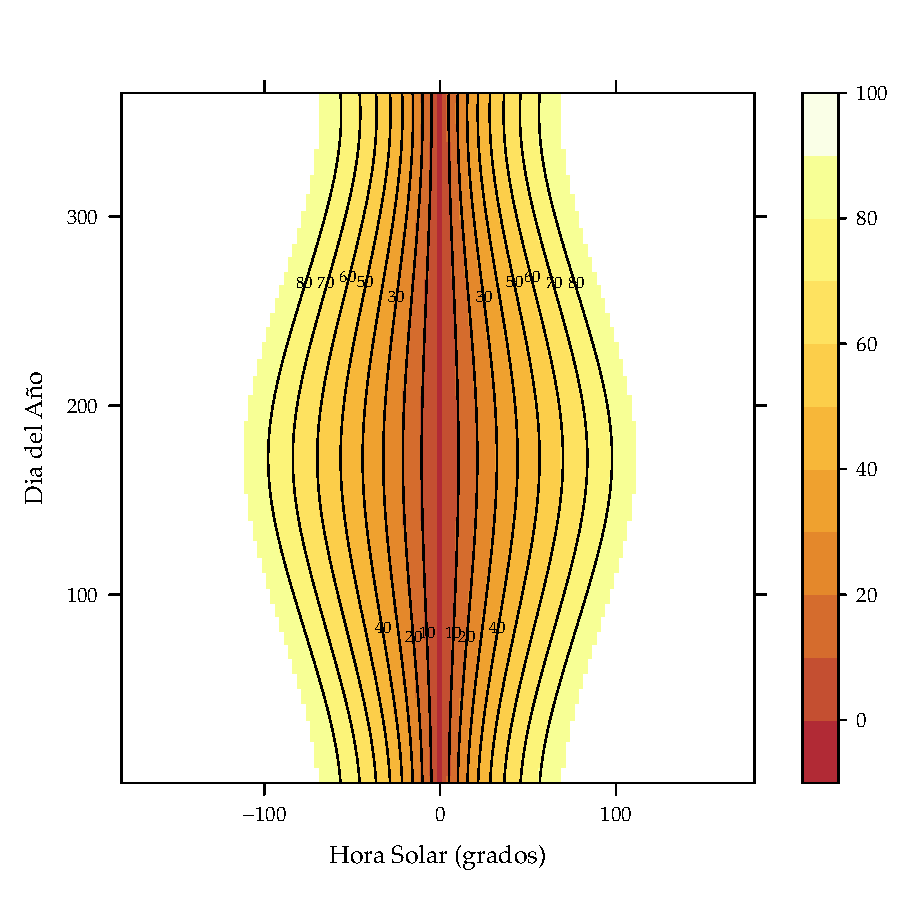
\includegraphics[height=0.85\textheight]{../figs/BetaHoriz_40N.pdf}
\end{center}
\end{frame}



\begin{frame}[label={sec:org7f95e5e}]{Ángulo de Incidencia Seguidor 1x NS}
\begin{itemize}
\item \(40\degree N\)
\end{itemize}
\begin{center}
\includegraphics[height=0.85\textheight]{../figs/cosThetaHoriz_40N.pdf}
\end{center}
\end{frame}




\begin{frame}[label={sec:org3a6a3ee},plain]{Ángulo de Incidencia Seguidor 2x}
\begin{columns}
\begin{column}{0.8\columnwidth}
\begin{center}
\includegraphics[height=0.8\textheight]{../figs/Sombra2X.pdf}
\end{center}
\end{column}

\begin{column}{0.2\columnwidth}
\begin{align*}
  \beta &= \theta_{z}\\
  \alpha &= \psi_{s}\\
  \cos(\theta_{s}) &= 1
\end{align*}
\end{column}
\end{columns}
\end{frame}
\begin{frame}[label={sec:orgfe82437}]{Inclinación Seguidor 2x}
\begin{itemize}
\item \(40\degree N\)
\end{itemize}
\begin{center}
\includegraphics[height=0.85\textheight]{../figs/BetaDoble_40N.pdf}
\end{center}
\end{frame}


\section{Radiación Efectiva según tipologías}
\label{sec:orgc4b8919}

\begin{frame}[label={sec:org7566347}]{Referencia: radiación en plano horizontal}
\begin{center}
\includegraphics[height=0.85\textheight]{../figs/G0yKrig.pdf}
\end{center}
\end{frame}


\begin{frame}[label={sec:org0d9766d}]{Radiación en Sistema estático}
\begin{center}
\includegraphics[height=0.85\textheight]{../figs/FixedKrig.pdf}
\end{center}
\end{frame}



\begin{frame}[label={sec:orgf03d7d8}]{Radiación en Seguimiento Eje Horizontal}
\begin{center}
\includegraphics[height=0.85\textheight]{../figs/HorizKrig.pdf}
\end{center}
\end{frame}



\begin{frame}[label={sec:org0c430c8}]{Radiación en Seguimiento Doble Eje}
\begin{center}
\includegraphics[height=0.85\textheight]{../figs/TwoKrig.pdf}
\end{center}
\end{frame}


\begin{frame}[label={sec:org93cdd50}]{Comparación Doble Eje-Estática}
\begin{center}
\includegraphics[height=0.85\textheight]{../figs/TwoFixed.pdf}
\end{center}
\end{frame}



\begin{frame}[label={sec:orgcd30d8b}]{Comparación Doble Eje - Horizontal}
\begin{center}
\includegraphics[height=0.85\textheight]{../figs/TwoHoriz.pdf}
\end{center}
\end{frame}



\begin{frame}[label={sec:orgf109851}]{Comparación Eje Horizontal - Estática}
\begin{center}
\includegraphics[height=0.85\textheight]{../figs/HorizFixed.pdf}
\end{center}
\end{frame}



\begin{frame}[label={sec:orgfeb0daa}]{Comparación entre Sistemas}
\begin{center}
\includegraphics[height=0.9\textheight]{../figs/compSystems.pdf}
\end{center}
\end{frame}

\begin{frame}[label={sec:org6bd6e20}]{Comparación entre Sistemas}
\begin{center}
\includegraphics[height=0.9\textheight]{../figs/compSystemsG0.png}
\end{center}
\end{frame}
\end{document}